%Zeitzauskommentiert %\edtext{
% %\begin{wrapfigure}{l}{0.3\textwidth}     
% \begin{center}         
%                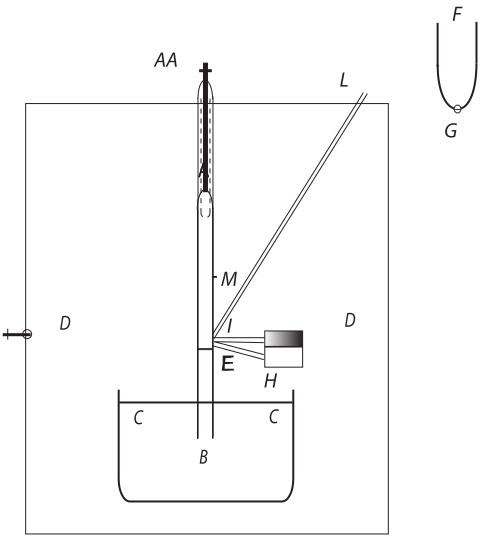
\includegraphics[width=0.6\textwidth]{images/37_3_103r1}\\ \textit{[Fig. 4]}\footnote{\textit{Der Tubus IL ist von Leibniz in der Bezeichnung ung\"{u}ltig gemacht, die Zeichnung im Text aber erhalten.}}
%                \end{center}
%                        %\caption{Bildbeschreibung}
%                %        \end{wrapfigure}
%                        %@ @ @ Dies ist eine Abstandszeile - fuer den Fall, dass mehrere figures hintereinander kommen, ohne dass dazwischen laengerer Text steht. Dies kann zu einer Fahlermeldung fuehren. @ @ @ \\
%                  %
             \startlock    [103~r\textsuperscript{o}]  \edlabel{tubusstart}Esto Tubus Torricellianus Mercurio plenus \textit{AB} cum vase subjecto \textit{C} eundem Mercurium  continente positus in vase aere clauso ordinario \edlabel{tubusend} pleno.
              % {\lemma{}\xxref{tubusstart}{tubusend}\Afootnote{ \textit{ (1) }\ 
          %     massae\protect\index{Sachverzeichnis}{massa|textit} aereae extra Tubum, Mercurio\protect\index{Sachverzeichnis}{mercurius|textit} suspenso  contraponderat, hinc eadem semper ejus altitudo,  quaecunque sit altitudo Tuborum. Hoc ut clarius  intelligatur Experimentum fiat in aqua  \textit{(aaaaa aaa)}\ sed Elastica,  qualis calida \textit{(bbbbb bbb)}\  seu quae comprimi potest, qualis  est calida, aut quae aerem habet immixtum \textit{ (5) }\ Esto Tubus Torricellianus\protect\index{Sachverzeichnis}{Tubus Torricellianus|textit}   \textbar\ \textit{AB} \textit{ erg.}\ \textbar\  cum vase subjecto   \textbar\ C. \textit{ erg.}\ \textbar\  positus in  \textit{(a)}\ aqua  \textit{(aa)}\ ponderis \textit{(bb)}\ tantae altitudinis, ut Mercurium\protect\index{Sachverzeichnis}{mercurius|textit} elevet  ad  \textit{(aaa)}\ tantam \textit{(bbb)}\ eandem altitudinem quae est Baroscopii\protect\index{Sachverzeichnis}{baroscopium|textit}:  \textit{(aaaa)}\ necesse est \textit{(bbbb)}\ \textit{BE} \textit{(cccc)}\ Reliquus Mercurius\protect\index{Sachverzeichnis}{mercurius|textit} \textit{(b)}\  vase clauso \textit{D} aere ordinario  pleno \textit{ (6) }\ . Esto Tubus Torricellianus   \textbar\ Mercurio plenus \textit{ erg.}\ \textbar\  \textit{AB}   \textbar\ cum \textit{ erg.}\ \textbar\  vase subjecto \textit{C}   \textit{(a)}\ positus eodem mercurio\protect\index{Sachverzeichnis}{mercurius|textit} ple  \textit{(b)}\ eundem [...] clauso  \textbar\ ordinario \textit{ erg.}\ \textbar\  pleno. \textit{ L}}}
                 Tubo \textit{AB} ita inverso, ut orificium \textit{B} perpendiculariter in Vas \textit{C} intret, Mercurius\protect\index{Sachverzeichnis}{mercurius} omnis e 
                 \endlock Tubo effluet, praeter altitudinem 27 circiter pollicum \textit{BE}. Hujus rei ratio est manifesta quia aer qui  est in \textit{D} \edtext{delapsu Mercurii ex Tubo \textit{AB} in vas \textit{D} necessario  comprimitur,}{\lemma{\textit{D}}\Afootnote{ \textit{ (1) }\ sustinere potest,  \textit{(a)}\ tantum \textit{(b)}\  quo  minus ultra statum   \textbar\ suum \textit{ erg.}\ \textbar\  ordinarium comprimatur  \textit{ (2) }\ delapsu [...] comprimitur, \textit{ L}}} vas \textit{D} enim omnem aerem quem habet  retinet, (neque enim in spatium relictum in Tubo \textit{AB} transferre potest) et praeterea Mercurium\protect\index{Sachverzeichnis}{mercurius}  accipit. Comprimitur ergo hoc delapsu aer in \textit{D} et aer per consequens in Tubo relictus \edtext{ex ipso Mercurio\protect\index{Sachverzeichnis}{mercurius purgatus} ab aere non purgato expressus}{\lemma{}\Afootnote{ex [...] expressus \textit{ erg.} \textit{ L}}} % \edtext{}{\lemma{expressus}\Bfootnote{Diese Zeichnung wurde mit Bleistift ausgef\"{u}hrt.}}
 proprio Elaterio\protect\index{Sachverzeichnis}{elaterium} se dilatat, cujus rei Experimentum sumi\footnote{\textit{In der rechten Spalte}: \textso{Exper. 8.}}  potest. Si vesica flaccida intra Tubum in \textit{A}  alligetur, ea enim Mercurio\protect\index{Sachverzeichnis}{mercurius} delapso sese \edtext{ipsa}{\lemma{}\Afootnote{ipsa \textit{ erg.} \textit{ L}}} inflabit,  seu tendet. Non ergo violenta est \edtext{ut autoribus funiculi\protect\index{Sachverzeichnis}{funiculus} videbatur}{\lemma{}\Afootnote{ut autoribus funiculi\protect\index{Sachverzeichnis}{funiculus} videbatur \textit{ erg.} \textit{ L}}} sed voluntaria  aeris in \textit{AB} relicti tensio\protect\index{Sachverzeichnis}{tensio}, nisi quatenus conjuncta  est cum ejus extra \textit{AB} in \textit{D} compressione, utique violenta.  Aer vero in \textit{D} hoc Mercurii\protect\index{Sachverzeichnis}{mercurius} delapsu comprimendus, resistet Elaterio\protect\index{Sachverzeichnis}{elaterium} suo. Elaterii\protect\index{Sachverzeichnis}{elaterium} enim duo sunt Effectus,  primum ut se dilatet, deinde ut resistat comprimenti,  prior effectus dici potest conatus\protect\index{Sachverzeichnis}{conatus} tensionis,  posterior resistentia compressionis. Conatus\protect\index{Sachverzeichnis}{conatus} tensionis  succedit aeri in \edtext{Tubo}{\lemma{}\Afootnote{ \textit{ (1) }\ Vase \textit{ (2) }\ Tubo \textit{ erg.} \textit{ L}}} \textit{AB} non succedit resistentia compressionis aeri in vase \textit{D}. Est enim resistentia  compressionis tanta \edtext{in aere ordinario}{\lemma{}\Afootnote{in aere ordinario \textit{ erg.} \textit{ L}}}, \edtext{ quantum est pondus}{\lemma{ordinario,}\Afootnote{ \textit{ (1) }\ quanta est vis ponderis  \textit{ (2) }\  quantum est pondus \textit{ L}}} massae\protect\index{Sachverzeichnis}{massa} aereae incumbentis. Quia ab ea non ultra  comprimi potest, quam in illum ipsum ordinarium  statum, quem nos in aere sentimus. Hinc quia ultra  ab ea comprimi non potest, non poterit etiam  comprimi ab eo quod ei massae\protect\index{Sachverzeichnis}{massa} aequiponderat, id est  a pollicibus Mercurii\protect\index{Sachverzeichnis}{mercurius} 27 \edtext{seu \textit{BE}.}{\lemma{}\Afootnote{seu \textit{BE} \textit{ erg.} \textit{ L}}} Sed quicquid praeterea Mercurii\protect\index{Sachverzeichnis}{mercurius} inerit \edtext{\textit{EA}}{\lemma{\textit{EA}}\Afootnote{ \textit{ erg.} \textit{ L}}}, illud\edtext{}{\lemma{}\Afootnote{illud  \textbar\ nihilo secius \textit{ gestr.}\ \textbar\ resistentiam \textit{ L}}} resistentiam  compressionis vincet et ex Tubo \textit{AB} in  vas \textit{D} delabens, \edtext{aerem vasis \textit{D} comprimet}{\lemma{delabens,}\Afootnote{ \textit{ (1) }\ tantumque comprimet  \textit{ (2) }\  aerem vasis \textit{D} comprimet \textit{ L}}}. Ut \edtext{sensu}{\lemma{}\Afootnote{sensu \textit{ erg.} \textit{ L}}} appareat aerem vasis \textit{D} esse  compressum hoc experimentum institui potest,\footnote{\textit{In der rechten Spalte}: \textso{Exper. 9.}} immittatur  ei vesica inflata, haec delapsu Mercurii\protect\index{Sachverzeichnis}{mercurius} fiet flaccida,  et tanto magis quanto plus Mercurii\protect\index{Sachverzeichnis}{mercurius} illapsum est seu quanto Mercurius\protect\index{Sachverzeichnis}{mercurius} est altior. Si quis putet aerem in \textit{AE}  relictum dilatatione vim pati, ad funiculum\protect\index{Sachverzeichnis}{funiculus} stabiliendum 